%
% Projekt:		DOKU: IFJ, IAL
% Autor:		Radek Pistelak, xpiste04@stud.fit.vutbr.cz 
%

\documentclass[a4paper, 11pt, titlepage]{article}
\usepackage[left=2cm,text={17cm,24cm},top=3cm]{geometry}
\usepackage[czech]{babel}
\usepackage[utf8]{inputenc}
\usepackage[IL2]{fontenc}

\usepackage{algorithmic}
\usepackage{graphicx}
\usepackage{hyperref}
\usepackage{wrapfig}

\usepackage{natbib}             % sazba pouzite literatury
\usepackage{url}                % sazba URL

\usepackage{url}
\usepackage{float}
\usepackage{listings}

\begin{document}

%%%%%%%%%%%%%%%%%%%%%%%%%%%%%%%%%%%%%%%%%%%%%%%%%%%%%%%%%%%%%%%%%%%%%%%%%
% ------ Titulní strana
%%%%%%%%%%%%%%%%%%%%%%%%%%%%%%%%%%%%%%%%%%%%%%%%%%%%%%%%%%%%%%%%%%%%%%%%%
\begin{titlepage}
\begin{center}
	\Large \textsc{Fakulta informačních technologií \\ Vysoké učení technické v~Brně} \\
	\vspace{\stretch{0.03}}

	%% logo FIT 
	\begin{figure}[h]
		\begin{center}
    		\scalebox{0.35}
    		{   
        		
\includegraphics{./img/logo.eps}
    		}
		\end{center}
	\end{figure}
	%%

	\vspace{\stretch{0.2}}
	Dokumentace do předmětu IMP k~projektu \\ \huge{MSP430: Voltmetr s vizualizací průběhu napětí pomocí VGA}  \\
	\vspace{\stretch{0.25}}

	\begin{center}
	{\Large \today}
	\end{center}

	\vspace{\stretch{0.618}}

	\noindent
	\begin{minipage}{0.4\textwidth}
		\begin{flushleft} \large
			Radek \textsc{Pištělák}
		\end{flushleft}
	\end{minipage}%
	\begin{minipage}{0.4\textwidth}
		\begin{flushright} \large
			\texttt{xpiste04@stud.fit.vutbr.cz}
		\end{flushright}
	\end{minipage}

\end{center}
\end{titlepage}

%%%%%%%%%%%%%%%%%%%%%%%%%%%%%%%%%%%%%%%%%%%%%%%%%%%%%%%%%%%%%%%%%%%%%%%%%
% ------ Titulní strana ---- end
%%%%%%%%%%%%%%%%%%%%%%%%%%%%%%%%%%%%%%%%%%%%%%%%%%%%%%%%%%%%%%%%%%%%%%%%%

%%%%%%%%%%%%%%%%%%%%%%%%%%%%%%%%%%%%%%%%%%%%%%%%%%%%%%%%%%%%%%%%%%%%%%%%%
% text dokumentace
%%%%%%%%%%%%%%%%%%%%%%%%%%%%%%%%%%%%%%%%%%%%%%%%%%%%%%%%%%%%%%%%%%%%%%%%%
\pagestyle{plain}
\pagenumbering{arabic}
\setcounter{page}{1}

% ----- Úvod ------
\section{Zadání} % (fold)
\label{sub:zadani}
	Navrhněte aplikaci, která umožní, aby FITkit fungoval jako jednoduchý voltmetr. 
	Pro demonstraci zapojte externí potenciometr, který umožní plynulou změnu měřeného 
	napětí v rozsahu 0-5 V. Měřenou hodnotu zpracujte AD převodníkem (pomocí periferie ADC12) a 
	zobrazte pomocí VGA displeje formou osciloskopu. Volbu referenčního napětí provádějte 
	automaticky dle velikosti měřeného napětí a specifikace AD převodníku. Zobrazení na VGA 
	rozhraní bude využívat jednoduchou grafiku, kterou lze převzít např. z hry Had.
% subsection zadani (end)

\section{Úvod} % (fold)
\label{sec:Uvod}
	Zadání říká, že bychom měli pomocí periferie ADC12 zpracovat hodnotu vstupního napětí
	v rozsahu $0-5V$. Převodník, ale akceptuje pouze hodnoty v intervalu 
	$0 - 2.5V$. Je tedy nutné vstupní napětí upravit do přípustného intervalu pomocí 
	napěťového děliče (viz. \cite{wiki:Delic}). 
% section Uvod (end)

\section{Popis ovládání} % (fold)
\label{sec:popis_ovladani}
	Aplikace neposkytuje žádné příkazy ovlivňující její běh. 
% section popis_ovladani (end)

\section{Schéma zapojení} % (fold)
\label{sec:schema_zapojeni}

	\begin{figure}[htbp]
		\centering
		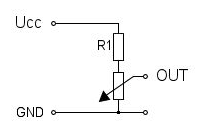
\includegraphics[width=0.25\textwidth]{img/c.png}
		\caption{Schéma zapojení}
	\end{figure}

			Kde \texttt{GND} je pin 39, \texttt{Ucc} pin 40 a \texttt{OUT} pin 37 na 
			FITkitu (v sekci MSP430). 

% section schema_zapojeni (end)

\section{Způsob řešení} % (fold)
\label{sec:implementace}
	Vlastní implementace je postavena nad aplikací \texttt{Snake} z \texttt{SVN} repozitáře
	FITkitu. Ze které je převzat kompletní \texttt{VHDL} kód a také kód pro grafické
	rozhraní na VGA displeji (\texttt{vga\_block.c} včetně hlavičkového souboru).

	Kód\footnote{\cite{320Volt:SampleCode}} pro práci s AD převodníkem byl 
	převzat ze stránek \url{http://320volt.com}
	a následně mírně upraven pro použití na platformě FITkit \citep{FITkit} i za 
	pomoci \citep{TI:UserGuide}.

	Zdrojové soubory \texttt{queue.h} a \texttt{print.h} jsou originální 
	a implementují kruhový buffer a funkce pro práci s ním.  

	Posledním souborem v řešení je pak \texttt{main.c}, který také vychází z aplikace
	\texttt{Snake} (přebírá z ní však pouze strukturu funkcí pro práci na platformě FITkit) 
	pak s pevně nastavenou frekvencí $33Hz$ (interval $30ms$) volá funkce pro získání
	hodnoty z AD převodníku a její výpis na LCD displej a také VGA displej. 

	Na LCD displej FITkitu je vypisována hodnota napětí zpracovaná AD převodníkem,
	která je vynásobena dvěmi. Napěťový dělič dělí napětí rovnoměrně (v případě maximální
	hodnoty potenciometru) a jelikož zadání požadovalo interval $0-5V$ byla hodnota zpětně upravena (i za cenu nepřesnosti). 
% section implementace (end)

\section{Závěr} % (fold)
\label{sec:zaver}
	Ve výsledné aplikaci není implementována změna referenčního napětí. Jinak je, ale 
	zadání splněno - FITkit zobrazuje průběh napětí na VGA displeji formou osciloskopu
	a také ``navíc'' zobrazuje přesnou hodnotu (v $mV$) na LCD displeji. 

	Jako pokračování práce by mohla být doimplementována podpora změny vzorkovací
	frekvence, nebo například funkce ``PAUSE'' pro pozastavení. Dalším možným 
	pokračováním by mohlo být také přepracování grafického rozhraní (na přesnější 
	s volitelnou mřížkou).  
% section zaver (end)

\newpage

\bibliographystyle{csplainnat}
\renewcommand{\refname}{Literatura}
\bibliography{literatura}

\pagestyle{empty}

\section*{Příloha A} % (fold)
\label{sec:prilohy}


\subsection{Výsledná aplikace} % (fold)
\label{sub:vysledna_aplikace}

\begin{figure}[htbp]
	\centering
	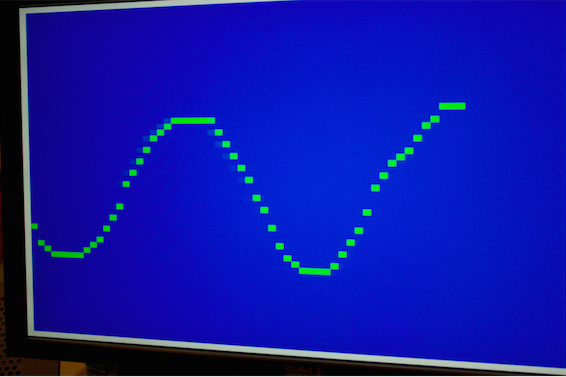
\includegraphics[width=0.95\textwidth]{img/b.png}
\end{figure}

% subsection vysledna_aplikace (end)

\newpage
\pagestyle{empty}

\section*{Příloha B} % (fold)
\label{sec:prilohy2}

\subsection{Výsledné zapojení} % (fold)
\label{sub:vysledne_zapojeni}

\begin{figure}[htbp]
	\centering
	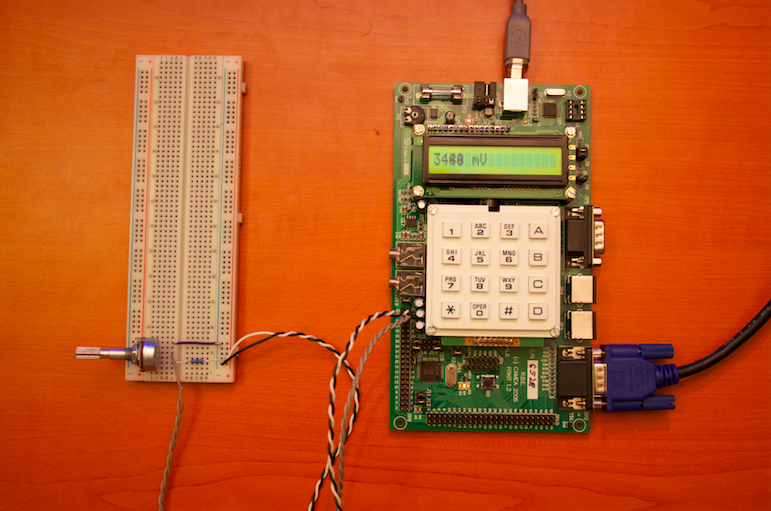
\includegraphics[width=0.95\textwidth]{img/a.png}
\end{figure}

% subsection vysledne_zapojeni (end)







\end{document}


